
\documentclass[11pt,en]{elegantpaper}

\title{Quantitative Risk Management Project 2}
\author{Qijun Yang \\ Duke University}
\institute{\href{https://fintech.meng.duke.edu}{Financial Technology of Duke}}
\version{1.0}
\date{Jan. 29, 2023}

% cmd for this doc
\usepackage{array}
\newcommand{\ccr}[1]{\makecell{{\color{#1}\rule{1cm}{1cm}}}}

\addbibresource[location=local]{reference.bib} % reference file
\begin{document}
\maketitle

\section*{\textcolor{orange}{Problem 1}}
Remember from last week we discussed that skewness and kurtosis functions in statistical packages 
are often biased. Is your function biased? Prove or disprove your hypothesis.

\section*{\textcolor{orange}{Answer}}
The python has both unbiased and biased estimator of skewness and kurtosis. The difference between the unbiased kurtosis estimator and the biased kurtosis estimator 
is significant. \textbf{The biased kurtosis estimator is biased when the sample size is small, 
but as the sample size increases, the biased kurtosis estimator becomes unbiased. Even though the result of the kurtosis estimator is reasonable, the difference 
between the unbiased skewness estimator and the biased skewness estimator is very small. 
Both are unbiased in the experiment.} There are some possible reasons for this, 
which I will discuss in the following analysis.

\subsection*{1. Background}
It is up to the user to decide whether the estimation of skewness and kurtosis in scipy, a Python package, 
is biased or not. There is a parameter called bias in the estimation function. It can be used to choose 
whether to use an unbiased estimator or not. If you set the bias to False, then the calculations will be 
corrected for the bias and the value that is calculated will be the adjusted Fisher-Pearson standardised 
coefficient of moments:
\[
    G_1=\frac{k_3}{k_2^{\frac{3}{2}}}=\frac{\sqrt{N(N-1)}}{N-2}\frac{m_3}{m_2^{\frac{3}{2}}}
\]

\subsection*{2. Experiment}
\textbf{Objection:} Test if the kurtosis and skewness calculated by scipy package is biased.

\textbf{Step:}
\begin{enumerate}[leftmargin = 70pt]
    \item Sample 5,10,100,100000 standardized random normal values separately.
    \item Calculate the kurtosis and skewness by setting bias to False and True separately.
    \item Sample the kurtosis and skewness by repeating <steps 1 and 2> 100 times.
    \item Calculate the first 2 moments of kurtosis and skewness, which are mean kurtosis  $\overline{\mu_k}$, 
    mean skewness $\overline \mu_{sk}$, standard deviation $\overline \sigma_k$,standard deviation $\overline \sigma_{sk}$.
    \item Set the significance level $\alpha=0.005$. Given the null hypotesis as $h\mu_k=0$ 
    and $\mu_{sk}=0$, calculate the T statistic of skewness and kurtosis separately. (T-test)
    \item Given the condition of two-side test, calculate the p-value of skewness and kurtosis.
    \item If the p-value is lower than significance level, then we reject the null hypotesis that skewness or kurtosis is unbiased.
\end{enumerate}

\subsection*{3. Results:}
\begin{enumerate}[leftmargin = 30pt]
    \item \textbf{Sample size = 5.}
    \begin{table}[h]
        \centering
        \caption{Sample moments of estimator When sample size = 5}
        \label{table1}
        \begin{tabular}{@{}cccccc@{}}
            \toprule
            \textbf{Characteristic} & \textbf{Description} & \textbf{Unbiased skewness}& \textbf{Unbiased kurtosis}& \textbf{Biased skewness} & \textbf{Biased kurtosis}\\
            \midrule
            Moments & Mean & -0.14544599 & 0.23005863 & -0.09756814 & -0.94248534 \\
            & Variance & 0.92341645 & 4.43911036 & 0.4155374 & 0.2774444 \\
            P-value & -- & 0.13332058 & 0.27751873 & 0.13332058 & 0.\\
            \bottomrule
        \end{tabular}
    \end{table}

    \item \textbf{Sample size = 10.}
    \begin{table}[h]
        \centering
        \caption{Sample moments of estimator When sample size = 10}
        \label{table2}
        \begin{tabular}{@{}cccccc@{}}
            \toprule
            \textbf{Characteristic} & \textbf{Description} & \textbf{Unbiased skewness}& \textbf{Unbiased kurtosis}& \textbf{Biased skewness} & \textbf{Biased kurtosis}\\
            \midrule
            Moments & Mean & -0.04352551 & -0.13300726 & -0.03670394 & -0.62069098 \\
            & Variance & 0.43281135 & 1.57664148 & 0.30777696 & 0.5044738 \\
            P-value & -- & 0.50976544 & 0.29205202 & 0.50976544 & 6.1284311e-14\\
            \bottomrule
        \end{tabular}
    \end{table}

    \subsubsection*{Reasoning}
    Let's first look at the unbiased skewness and the biased skewness. We can see that although their means 
    are different, their p-values are the same and both are above the significant level, which means that 
    we should accept the null hypothesis. They are statistically unbiased. However, this contradicts our 
    past experience and doesn't make sense.
    \newline
    \textbf{Firstly}, I'm inclined to attribute such a confusing result to rounding error, because the sample means 
    of unbiased and biased skewness are too close for the computer to differentiate their p-values.
    \newline
    \textbf{Secondly}, we get a sample from a standard normal distribution, which means that the sample is a 
    random variable. Its randomness leads to the randomness of the p-value. Therefore, such a result could 
    be just a coincidence. Therefore, I did some additional experiments and I find that the majority of 
    p-value is greater than the significant level.
    \newline
    \textbf{Third}, the distribution of the unbiased skewness estimator and the biased skewness estimator is not normal.
     T-test requires its random variable to be normal or approximately normal. If its random variable does 
     not fulfil such condition, then T-test requires large sample to make the statistic close to 
     t-distribution. In fact, under these circumstances, the distribution is asymptotically normal. However, 
     our sample size is only 5 and 10, which would reduce the efficiency of the t-test. In addition, the result is 
     not very precise and not very stable.

     Then we focus on the unbiased kurtosis and the biased kurtosis. We could quickly find that the mean of those 
     two are more different and their p-value obviously suggest that unbiased kurtosis estimator are unbiased,
     biased kurtosis estimator are biased.


     \item \textbf{Sample size = 100.}
     \begin{table}[h]
        \centering
        \caption{Sample moments of estimator When sample size = 100}
        \label{table3}
        \begin{tabular}{@{}cccccc@{}}
            \toprule
            \textbf{Characteristic} & \textbf{Description} & \textbf{Unbiased skewness}& \textbf{Unbiased kurtosis}& \textbf{Biased skewness} & \textbf{Biased kurtosis}\\
            \midrule
            Moments & Mean & -0.01493056 & 0.01284804 & -0.01470566 & -0.04719138 \\
            & Variance & 0.05716795 & 0.20712172 & 0.05545869 & 0.18720098 \\
            P-value & -- & 0.53376663 & 0.77829632 & 0.53376663 & 0.27804886\\
            \bottomrule
        \end{tabular}
    \end{table}

    \item \textbf{Sample size = 100000.}
    \begin{table}[h]
       \centering
       \caption{Sample moments of estimator When sample size = 100000}
       \label{table4}
       \begin{tabular}{@{}cccccc@{}}
           \toprule
           \textbf{Characteristic} & \textbf{Description} & \textbf{Unbiased skewness}& \textbf{Unbiased kurtosis}& \textbf{Biased skewness} & \textbf{Biased kurtosis}\\
           \midrule
           Moments & Mean & -0.00150312 & 0.00083446 & -0.0015031 & -0.00077442 \\
           & Variance & 6.09705474e-05 & 0.00022669 & 6.09705474e-05 & 0.00022667 \\
           P-value & -- & 0.05709829 & 0.58067351 & 0.05709829 & 0.60813631\\
           \bottomrule
       \end{tabular}
   \end{table}

   \subsubsection*{Reasoning}
   As we can see, the biased estimator tends to converge to the unbiased estimator as the sample size increases. 
   The variance of the biased and unbiased estimators decreases a lot and their mean is very close. Moreover, 
   their p-values are all above the significant level, so we could consider both as unbiased.
\end{enumerate}

\subsection*{4. Conclusion}

\textbf{When the sample size is small}, The kurtosis estimator behaves as expected, but the skewness estimator does not. 
An unbiased kurtosis estimator is statistically significant in unbias and a biased kurtosis estimator is biased. 
For skewness, both are unbiased, but I will attribute this to rounding error and small sample size.
\textbf{When the sample size is large}, the biased estimator converge to unbiased estimator and biasedness disappears.



\section*{\textcolor{orange}{Problem 2}}
\begin{enumerate}
    \item Fit the data in problem2.csv using OLS and calculate the error vector. Look at its distribution. 
    How well does it fit the assumption of normally distributed errors?
    \item Fit the data using MLE given the assumption of normality. 
    Then fit the MLE using the assumption of a T distribution of the errors. Which is the best fit?
    \item What are the fitted parameters of each and how do they compare? 
    What does this tell us about the breaking of the normality assumption in regards to expected values in this case?
\end{enumerate}

\section*{\textcolor{orange}{Answer}}

\subsection*{Problem 2.1}

\textbf{The residuals produced by OLS is not normally distributed.}

\subsubsection*{reasoning}

Given the dataset, we use OLS to fit the data and here is our reslut:

\begin{figure}[h] 
    \centering 
    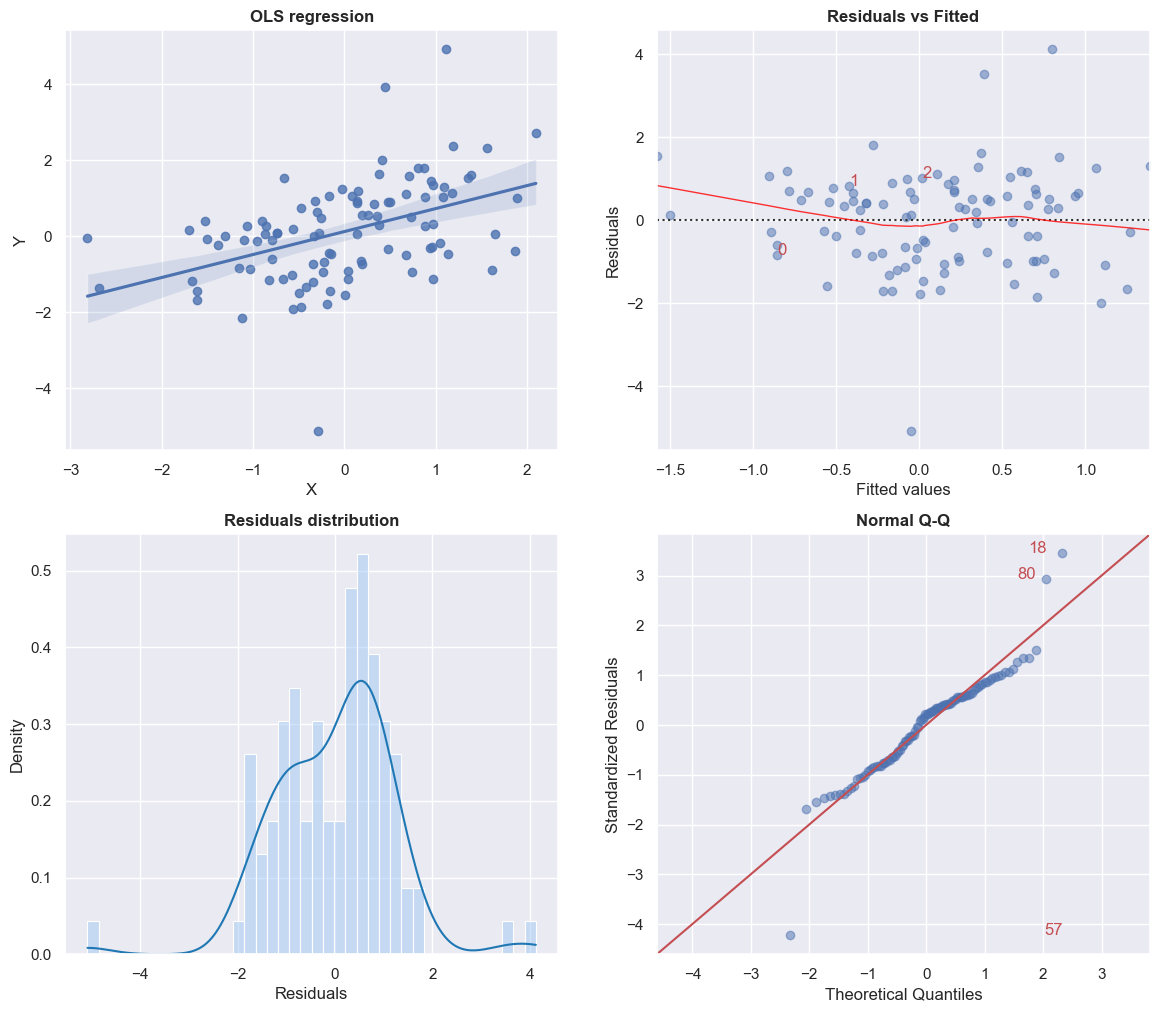
\includegraphics[width=0.8\textwidth]{./image/reg} 
\end{figure}

Now let's focus on the distribution of the residuals. We might find that it is more likely 
to be a left skewed distribution than a normal distribution. With such a guess, we could 
see that the Q-Q plot also shows that the residuals want to leave the diagonal line when 
they are away from 0.

With a visual check, we could now perform a normal test on the residuals. We use a method 
based on D'Agostino and Pearson's test, which combines skewness and kurtosis to produce an 
omnibus test of normality. And we find that the p-value = 0.0008475313945909529, which is 
less than our expected significance level of 0.05. We therefore reject the null hypothesis. 
The residuals are not normally distributed.


\subsection*{Problem 2.2}
\textbf{The MLE assuming T-distribution of error terms is better than that assuming normality.}

\subsubsection*{reasoning}


First, we use MLE assuming the normality of errors to fit the data. Then, assuming that 
the error term is T-distributed, we use MLE to run the regression. We could get the corresponding
parameters for each MLE and we use them to caculate the residuals. Here are some visuals for
residuals distribution and linear moded:

\begin{figure}[h] 
    \centering 
    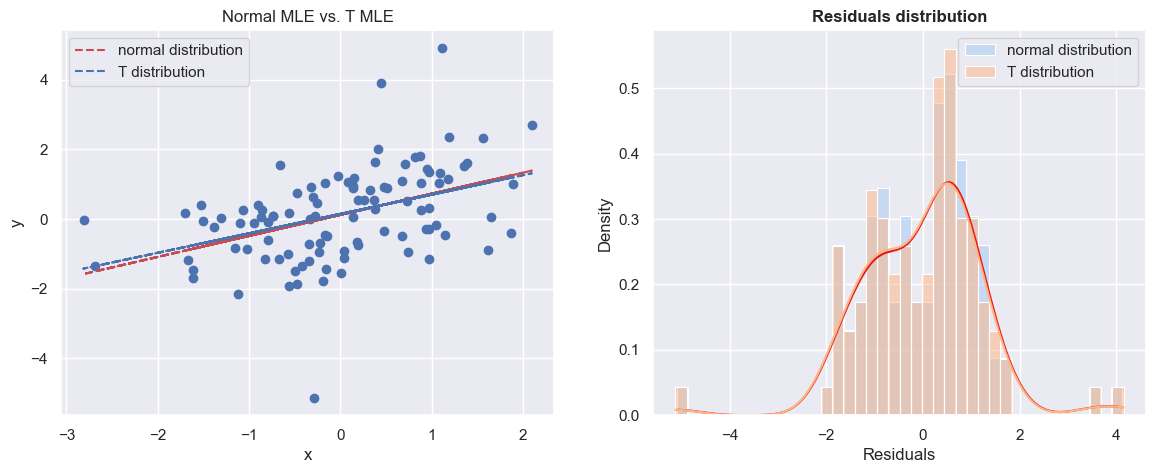
\includegraphics[width=1\textwidth]{./image/MLE} 
\end{figure}

From the images above, we could see that the difference between these two MLE is not very large 
and their residuals have a large amount of overlap. As a result, it is not easy to tell from 
the image which of the MLE is the better one. One interesting thing is that when we use MLE given 
error is T distributed, its residuals are still not normal distribution. It seems more left biased
distributed.

Now, let's look at some useful numbers. Even though direct images could not help us figure out which 
is better, those numbers may give us some reasonable explanation that T is more suitable for regression
this time.

Assuming that the error term is T-distributed, by MLE we could get the following results:

\begin{table}[h]
    \centering
    \caption{MLE under normal error assumption}
    \label{table5}
    \begin{tabular}{@{}ccc@{}}
        \toprule
        \textbf{Characteristic} & \textbf{Description} & \textbf{Value}\\
        \midrule
        Parameter & $\beta_1$ & 0.6052 \\
        & $\beta_0$ & 0.1198 \\
        & Variance  & 1.1984 \\
        Goodness of fit & $R^2$ & 0.1946 \\
        & $adjusted\  R^2$ & 0.1864 \\
        Information Criteria & AIC & 323.9841 \\
        & BIC & 329.1945\\
        \bottomrule
    \end{tabular}
\end{table}

Assuming that the error term is T-distributed, by MLE we could get the following results:

\begin{table}[h]
    \centering
    \caption{MLE under T error assumption}
    \label{table6}
    \begin{tabular}{@{}ccc@{}}
        \toprule
        \textbf{Characteristic} & \textbf{Description} & \textbf{Value}\\
        \midrule
        Parameter & $\beta_1$ & 0.5576 \\
        & $\beta_0$ & 0.1426 \\
        & Degree of freedom  & 6.2766 \\
        & Variance & 0.9713 \\
        Goodness of fit & $R^2$ & 0.1931 \\
        & $adjusted\  R^2$ & 0.1849 \\
        Information Criteria & AIC & 314.9459 \\
        & BIC & 320.1563 \\
        \bottomrule
    \end{tabular}
\end{table}

The $R^2$ and $adjusted\  R^2$ of those two MLE are very same, but the AIC and BIC of T-MLE is smaller that
Normal-MLE. Therefore, we could conclude that T-MLE is better for regression this time.

\subsection*{Problem 2.3}
\textbf{Not all error terms follow a normal distribution in our normal life. We could use different 
assumptions about error terms and compare their AIC, BIC or other statistics to see which one 
is more reasonable.}

\subsubsection*{reasoning}
If error follows a normal distribution:
\[y=0.1198+0.6052x+\epsilon, \qquad \epsilon \sim N(0,1.1984)\]

If error follows a T distribution:
\[y=0.1426+0.5576x+\epsilon, \qquad \epsilon \sim T(6.2766,0,0.9713)\]

From \textbf{Problem 2.2}, we could see T distribution is better.

\section*{\textcolor{orange}{Problem 3}}
Simulate AR(1) through AR(3) and MA(1) through MA(3) processes. Compare their ACF and PACF 
graphs. How do the graphs help us to identify the type and order of each process?

\section*{\textcolor{orange}{Answer}}

\subsection*{1. AR Process}
For AR model, we choose to simulate the following process:
\[x_t=0.75+0.4x_t-1+\epsilon, \qquad \epsilon \sim N(0,0.8)\]
\[x_t=0.75+0.4x_t-1+0.3x_{t-2}+\epsilon, \qquad \epsilon \sim N(0,0.8)\]
\[x_t=0.75+0.2x_t-1+0.3x_{t-2}+0.2x_{t-3}+\epsilon, \qquad \epsilon \sim N(0,0.8)\]

Meanwhile, we calculate and plot the autocorrelation function (ACF) and the partial 
autocorrelation function (PACF). We can easily see that for the AR(1) model, the PACF 
becomes insignificant after the first lag; for the AR(2) model, the PACF becomes 
insignificant after the second lag; for the AR(3) model, the PACF becomes insignificant 
after the third lag. Their ACF also falls to zero or becomes insignificant more slowly. 
\textbf{Therefore, we can safely conclude that the PACF of the AR(p) model would become 
insignificant after the $p^{th}$ lag and its ACF would slowly converge to zero.}


\begin{figure}[htbp] 
    \centering 
    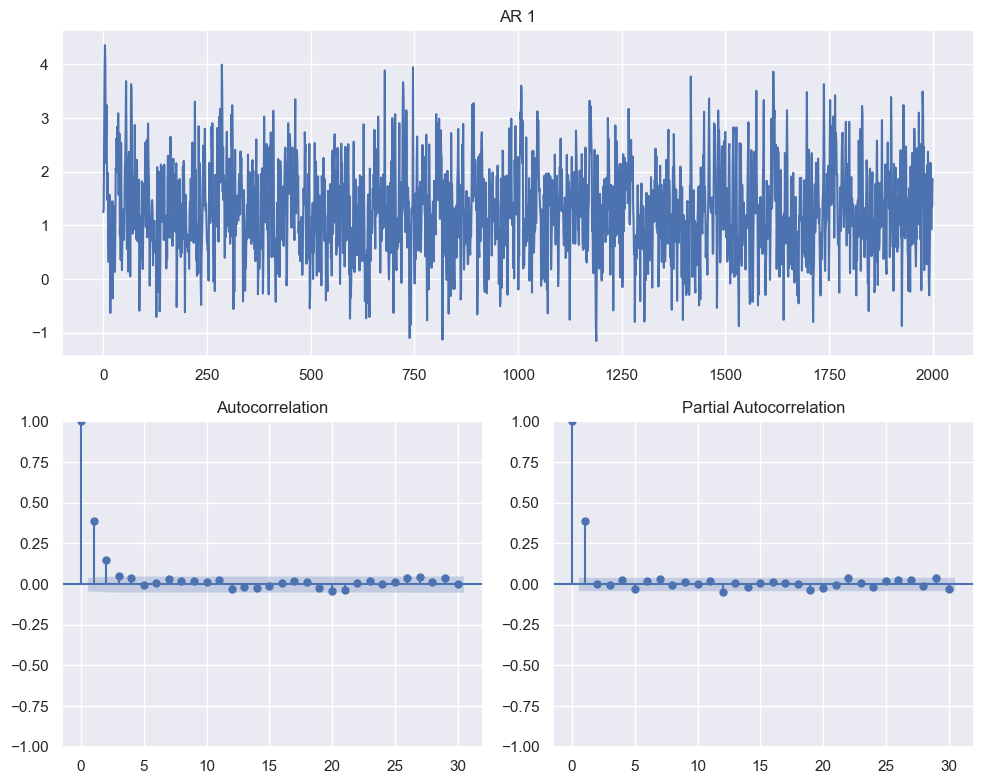
\includegraphics[width=0.65\textwidth]{./image/AR1} 
\end{figure}

\begin{figure}[htbp] 
    \centering 
    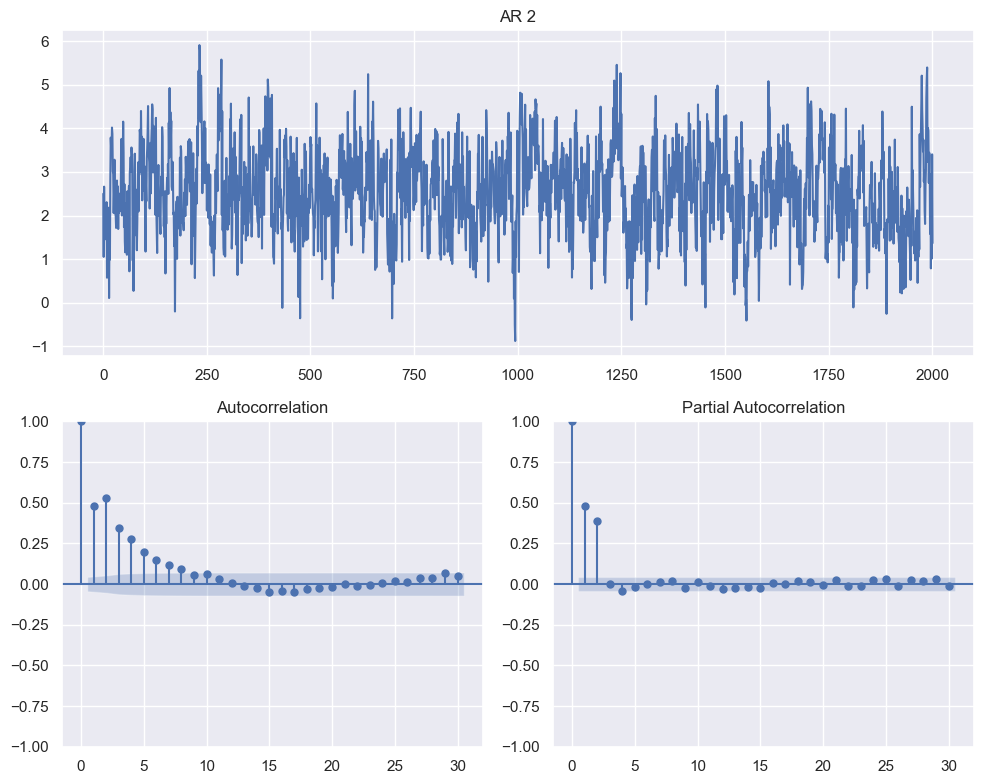
\includegraphics[width=0.7\textwidth]{./image/AR2} 
\end{figure}
\begin{figure}[htbp] 
    \centering 
    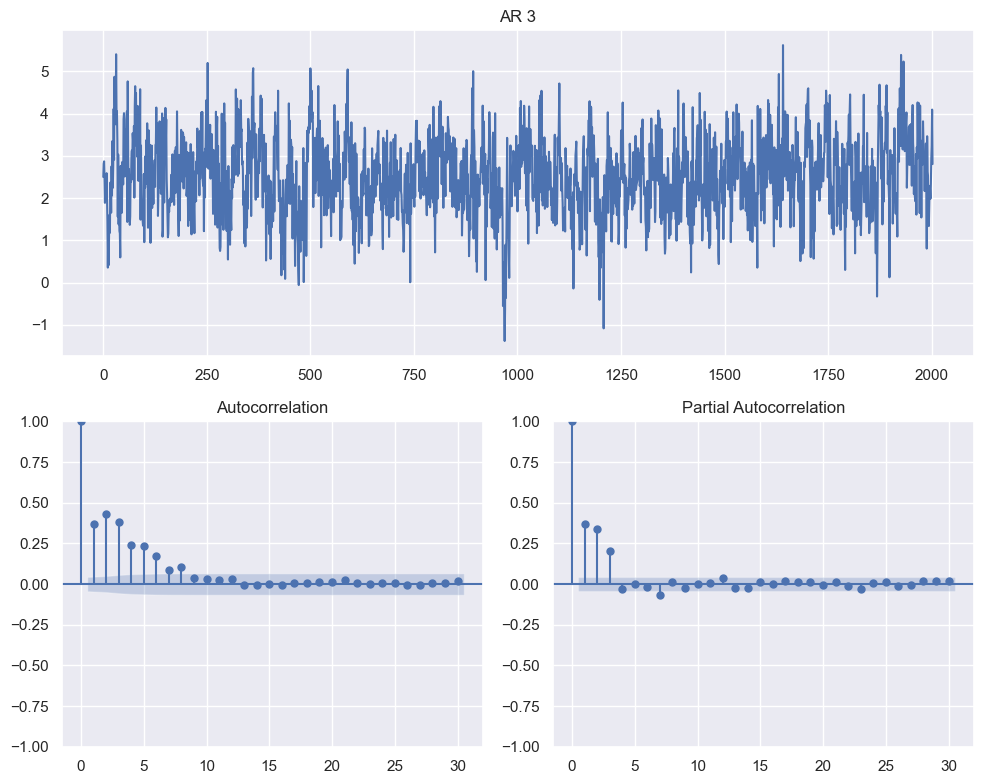
\includegraphics[width=0.7\textwidth]{./image/AR3} 
\end{figure}

\subsection*{2. MA Process}


For AR model, we choose to simulate the following process:
\[x_t=0.75+\epsilon_t+0.4\epsilon_{t-1}, \qquad \epsilon_i \sim N(0,0.8)\]
\[x_t=0.75+\epsilon_t+0.4\epsilon_{t-1}+0.3\epsilon_{t-2}, \qquad \epsilon_i \sim N(0,0.8)\]
\[x_t=0.75+\epsilon_t+0.2\epsilon_{t-1}+0.3\epsilon_{t-2}+0.2\epsilon_{t-3}, \qquad \epsilon_i \sim N(0,0.8)\]

Also, ACF and PACF are calculated and plotted. From the following figures, we can find that
The ACFs are not significant after the first lag for MA(1), after the second lag for 
MA(2) and after the third lag for MA(3). However, there is no obvious pattern about PACF.
\textbf{Therefore, for MA(q) model, we could guess their oder by looking at ACF. If its $q^{th}$ lag
of ACF becomse insignificant and its PACF slowly converge to zero, then it has great possibility to be MA(q)
}
\begin{figure}[htbp] 
    \centering 
    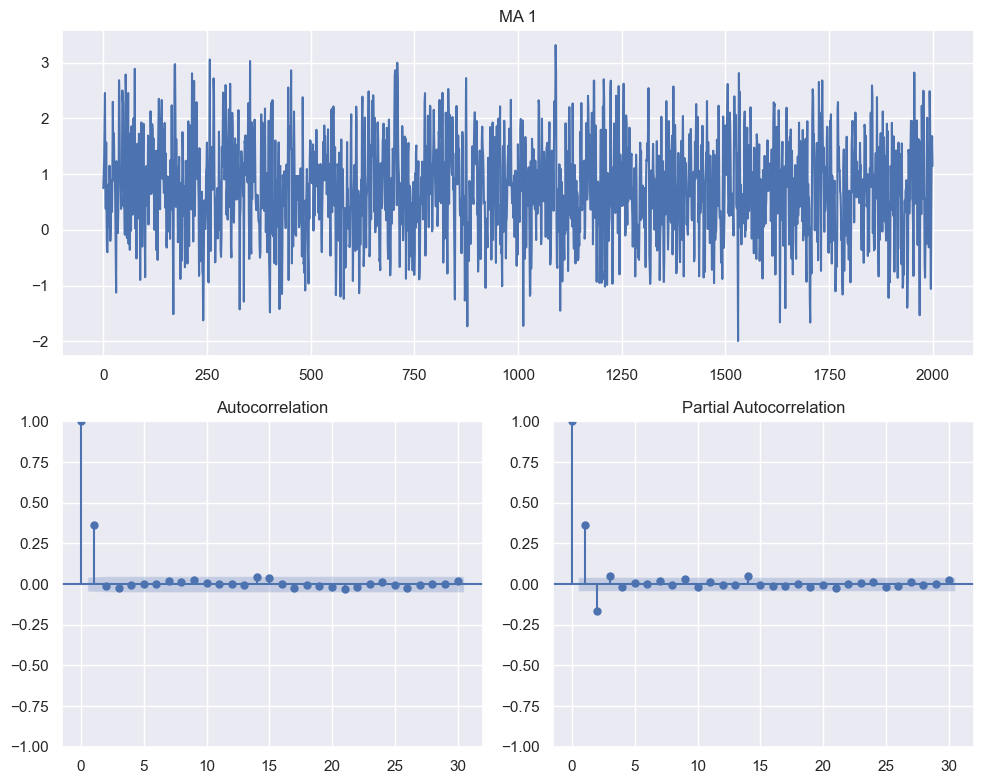
\includegraphics[width=0.7\textwidth]{./image/MA1} 
\end{figure}

\begin{figure}[htbp] 
    \centering 
    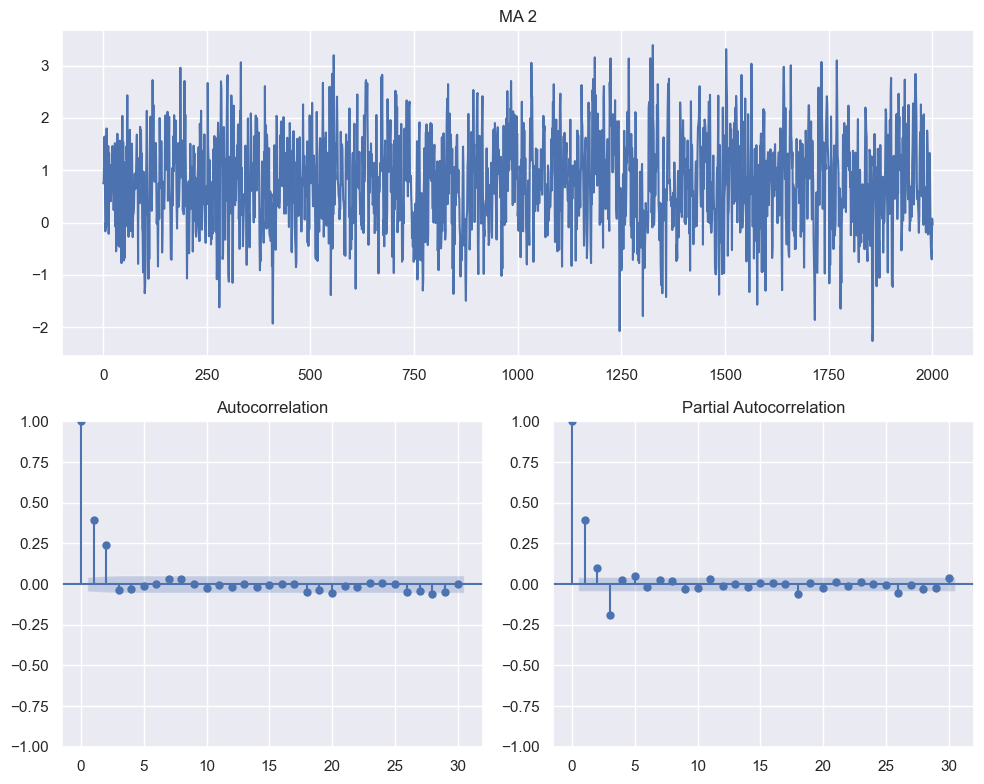
\includegraphics[width=0.7\textwidth]{./image/MA2} 
\end{figure}
\begin{figure}[htbp] 
    \centering 
    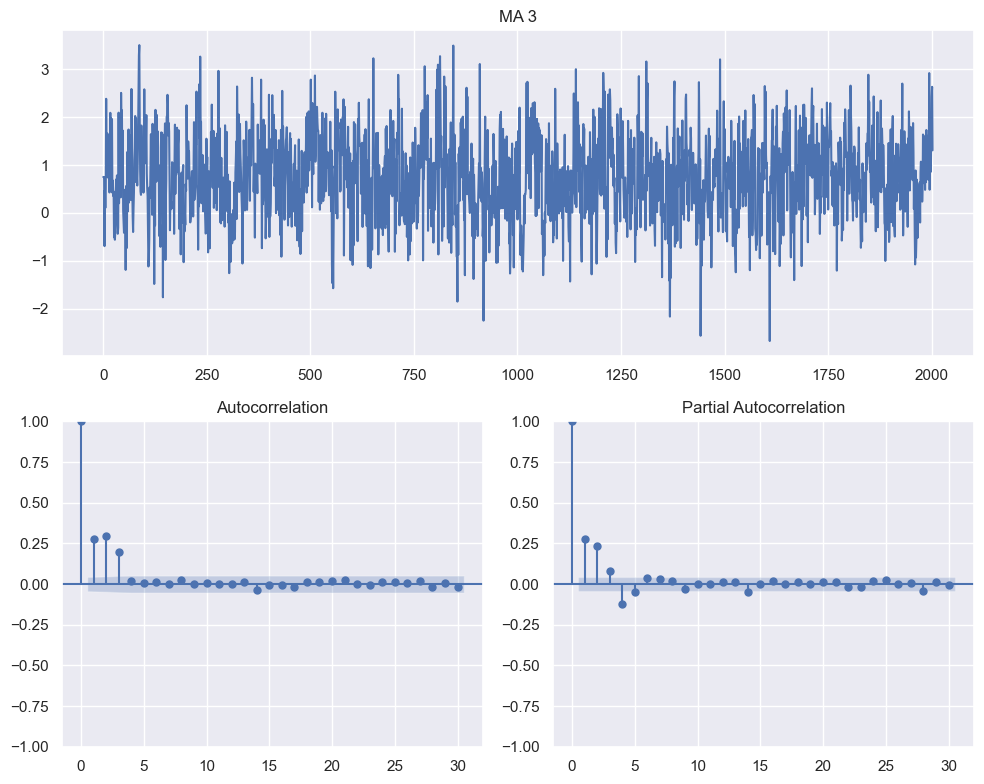
\includegraphics[width=0.7\textwidth]{./image/MA3} 
\end{figure}


\newpage
\section*{\textcolor{orange}{Feedback}}

\begin{enumerate}
    \item Full Credit
    \item Full Credit
    \item -0.25 I would suggest using python package, some of your graph seems wrong(MA(3) for example)
        \textcolor{brown}{ \begin{enumerate}
            \item \textbf{AR: } abs(ACF) for AR is always non-zero, decaying through time.  PACF for AR is only non-zero
            for the number of lags in the model.
            \item \textbf{MA: }ACF for MA is only non-zero for the number of lags in the model. abs(PACF) for MA decays through time.
        \end{enumerate}
        }
        See the formuals for autocovariance (which is scaled correlation) in the notes.(\textbf{Feixed my code bugs.})
\end{enumerate}
\end{document}